\documentclass[tikz]{standalone}
\usepackage{tikz}
\usetikzlibrary{positioning, shapes.multipart, arrows, shadows, backgrounds, fit}
\usepackage{amsmath}
\usepackage{amssymb}
\usepackage{amsthm}
\tikzset{
	WL/.style={
		draw,
		rectangle,
		minimum height=2.4cm,
		text width = .15cm,
		fill=cyan,
		align=center,
		inner sep=2ex
	},
}
\usetikzlibrary{decorations.shapes}
\newcommand{\fillcolor}{cyan!70!black}
\newcommand{\fillcolorgreen}{green!70!black}
\newcommand{\boundarycolor}{black}
\tikzset{decorate sep/.style 2 args=
	{decorate,decoration={shape backgrounds,shape=circle,shape size=#1,shape sep=#2}}}


\usetikzlibrary{fadings,shapes.arrows,shadows}   
\usetikzlibrary{calc,tikzmark}

\newcommand{\vc}[1]{{\color{magenta!80!black}#1}}
\newcommand{\wc}[1]{{\color{blue}#1}}
\renewcommand{\d}{\text{\sffamily{d}}}

\tikzfading[name=arrowfading, top color=transparent!0, bottom color=transparent!95]
\tikzset{arrowfill/.style={top color= black!20, bottom color=black, text= white, general shadow={fill=black, shadow yshift=-0.8ex, path fading=arrowfading}}}
\tikzset{arrowstyle/.style={draw=black,arrowfill, single arrow,minimum height=#1, single arrow,
		single arrow head extend=.4cm,}}

\newcommand{\tikzfancyarrow}[2][2cm]{\tikz[baseline=-0.5ex]\node [arrowstyle=#1] {#2};}

\newcommand{\rk}{{\sffamily{RK4}}}

\usepackage{color}
\definecolor{bluegreen}{rgb}{0.0, 0.87, 0.87}
\usetikzlibrary{fadings,shapes.arrows,shadows}   
\usetikzlibrary{shapes.multipart}

\tikzfading[name=arrowfading, top color=transparent!0, bottom color=transparent!95]
\tikzset{arrowfill/.style={top color= black!20, bottom color=orange, general shadow={fill=black, shadow yshift=-0.8ex, path fading=arrowfading}}}
\tikzset{arrowstyle/.style={draw=black,arrowfill, single arrow,minimum height=#1, single arrow,
		single arrow head extend=.4cm,}}


\begin{document}
	\tikzstyle{sum} = [draw = red!50!black, fill=cyan, circle=.1cm, node distance=.5cm]
	\begin{tikzpicture}[font=\sffamily]
		\node[ fill = white,draw = green!50!black, text = black, thick,rounded corners = 0.5ex] (burger) {\begin{tabular}{c}
				{\color{red!30!black} \huge Noisy data}  \\ 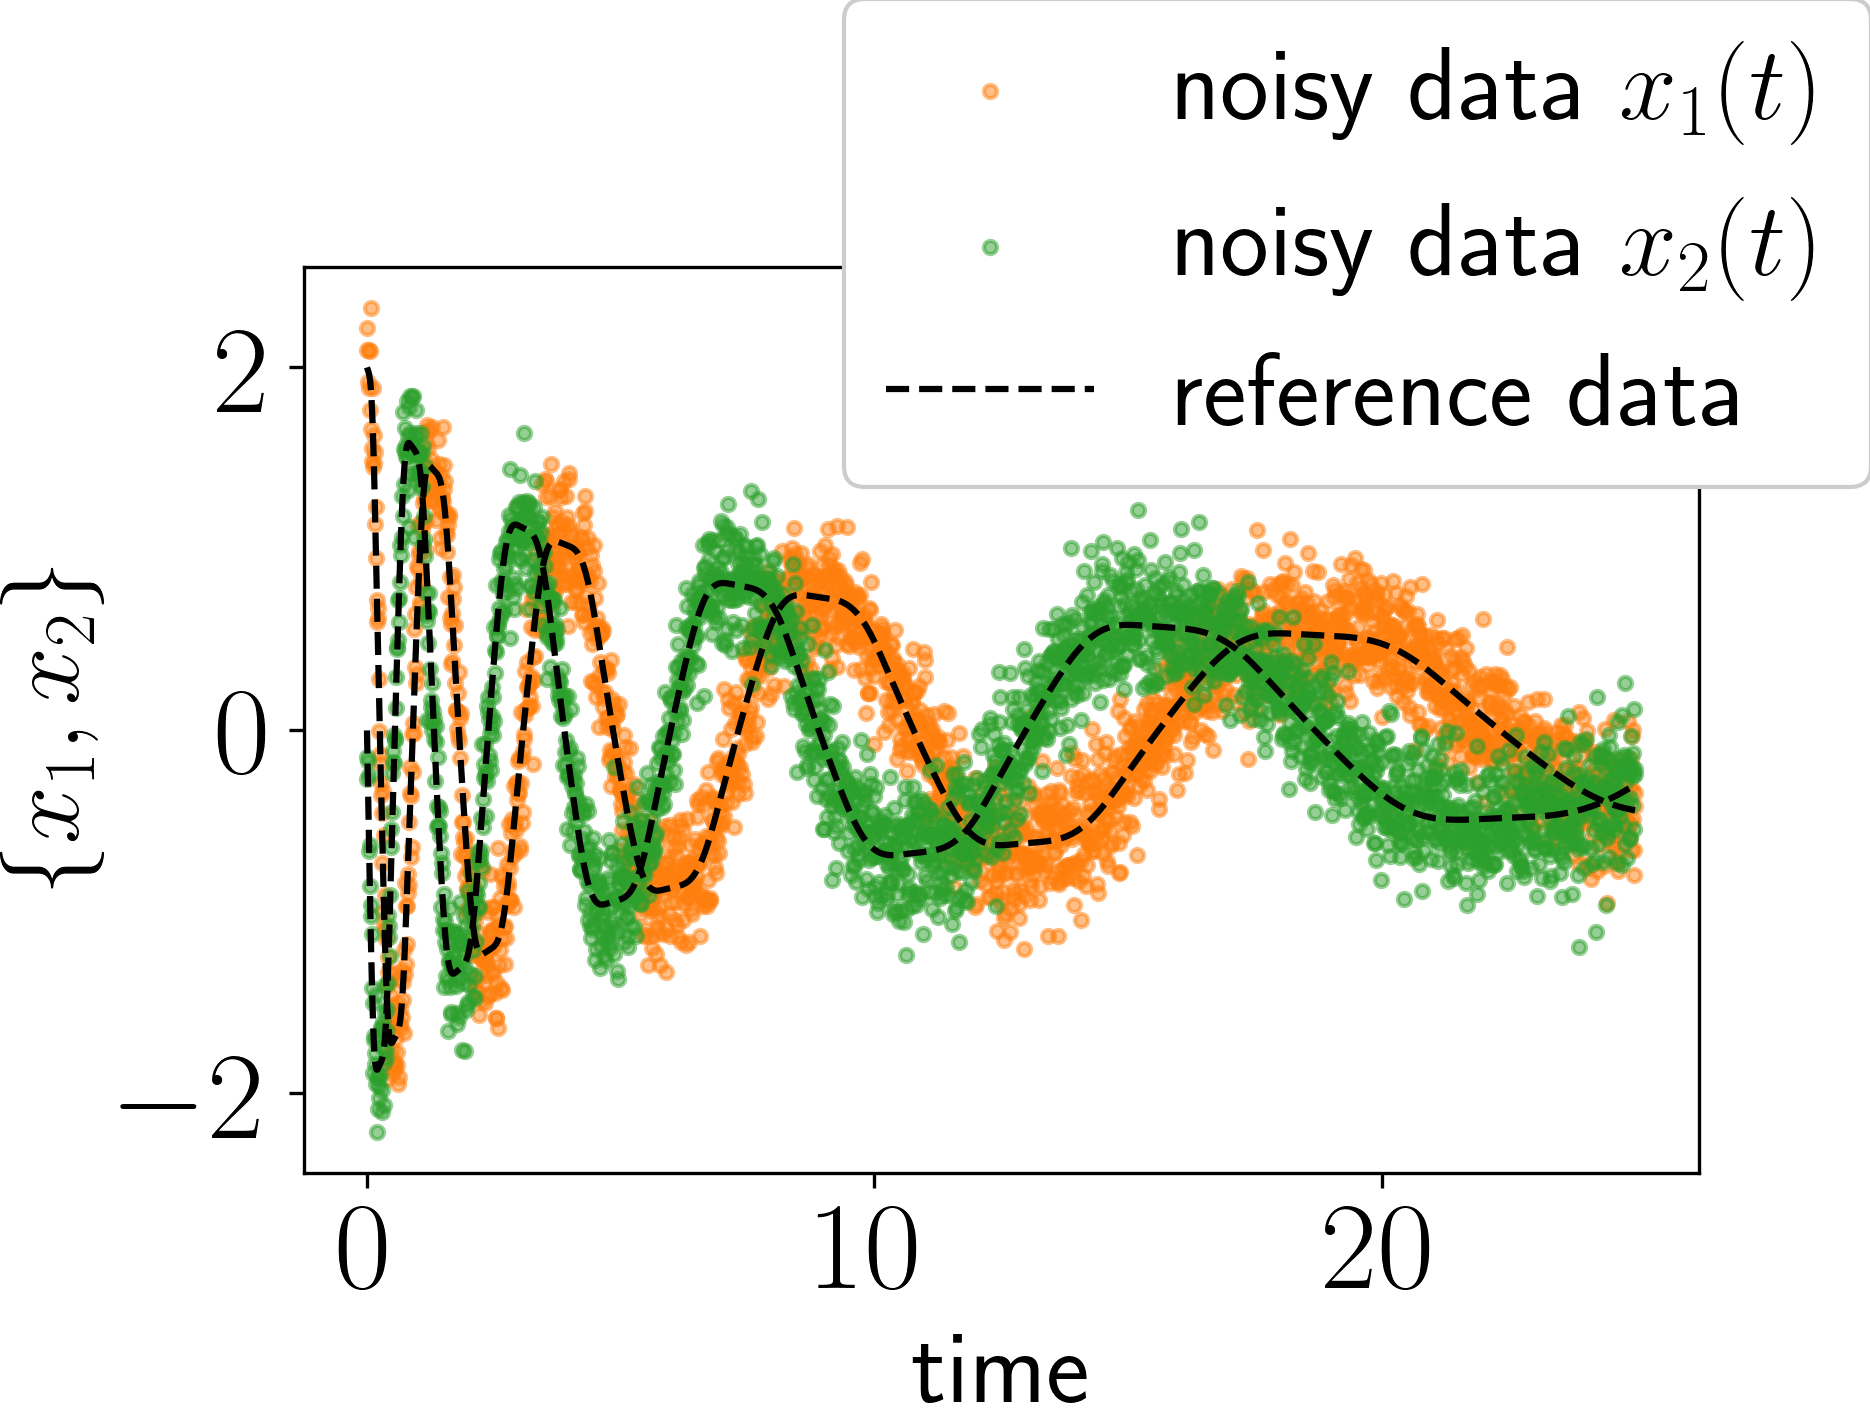
\includegraphics[trim = 0cm 0.cm 0.cm 0cm, clip, height = 4.5cm]{./main_diag1.pdf}
		\end{tabular}};
		% Implicit part
		\node[ fill = white,draw = green!50!black, below right = 0cm and 6cm of burger.north, text = black, thick,rounded corners = 0.5ex] (implicit_respresentation) {
			\begin{tabular}{c}
				{\color{red!30!black} \huge Learning implicit representation and governing equations} \\[5pt]
				%	\includegraphics[scale = 1.0]{Implicit_respresentation.pdf}
				\begin{tikzpicture}[cir/.style={circle,draw=#1,minimum size=0.5},y=1cm,font=\sffamily, inner sep=7,transform shape,scale=1.0]
					\begin{scope}[rotate=0, scale = 0.8]
						\draw[draw=\fillcolor, opacity=0.4, thick, rounded corners=.1cm, fill = cyan!10!white ] (-0.75,-4.8) rectangle ++(7.5,5.2);
						%%
						\node[cir=black,fill=cyan!50!black, draw = \boundarycolor, ultra thick] (I1) at (-2,-1) {};
						\node[cir=black,fill=cyan!50!black,draw = \boundarycolor,ultra thick] (I2) at (-2,-2) {};
						\node[cir=black,fill=cyan!50!black,draw = \boundarycolor,ultra thick] (I3) at (-2,-3) {};

						%%
						\node[cir=black,fill=\fillcolor, opacity=0.4,draw = \boundarycolor,ultra thick] (a1) at (0,0) {};
						\node[cir=black,fill=\fillcolor, opacity=0.4,draw = \boundarycolor,ultra thick] (a2) at (0,-1) {};
						\node[cir=black,fill=\fillcolor, opacity=0.4,draw = \boundarycolor,ultra thick] (a3) at (0,-2) {};
						\node[cir=black,fill=\fillcolor, opacity=0.4,draw = \boundarycolor,ultra thick] (a4) at (0,-3) {};
						\node[cir=black,fill=\fillcolor, opacity=0.4,draw = \boundarycolor,ultra thick] (a5) at (0,-4) {};
						%%
						\node[cir=cyan!50!black,fill=\fillcolor, opacity=0.4,draw = \boundarycolor,ultra thick] (b1) at (2,0) {};
						\node[cir=cyan!50!black,fill=\fillcolor, opacity=0.4,draw = \boundarycolor,ultra thick] (b2) at (2,-1) {};
						\node[cir=cyan!50!black,fill=\fillcolor, opacity=0.4,draw = \boundarycolor,ultra thick] (b3) at (2,-2) {};
						\node[cir=cyan!50!black,fill=\fillcolor, opacity=0.4,draw = \boundarycolor,ultra thick] (b4) at (2,-3) {};
						\node[cir=cyan!50!black,fill=\fillcolor, opacity=0.4,draw = \boundarycolor,ultra thick] (b5) at (2,-4) {};
						%%
						\node[cir=cyan!50!black,fill=\fillcolor, opacity=0.4,draw = \boundarycolor,ultra thick] (c1) at (4,0) {};
						\node[cir=cyan!50!black,fill=\fillcolor, opacity=0.4,draw = \boundarycolor,ultra thick] (c2) at (4,-1) {};
						\node[cir=cyan!50!black,fill=\fillcolor, opacity=0.4,draw = \boundarycolor,ultra thick] (c3) at (4,-2) {};
						\node[cir=cyan!50!black,fill=\fillcolor, opacity=0.4,draw = \boundarycolor,ultra thick] (c4) at (4,-3) {};
						\node[cir=cyan!50!black,fill=\fillcolor, opacity=0.4,draw = \boundarycolor,ultra thick] (c5) at (4,-4) {};
						%%
						\node[cir=cyan!50!black,fill=\fillcolor, opacity=0.4,draw = \boundarycolor,ultra thick] (d1) at (6,0) {};
						\node[cir=\boundarycolor,fill=\fillcolor, opacity=0.4,draw = \boundarycolor,ultra thick] (d2) at (6,-1) {};
						\node[cir=\boundarycolor,fill=\fillcolor, opacity=0.4,draw = \boundarycolor,ultra thick] (d3) at (6,-2) {};
						\node[cir=\boundarycolor,fill=\fillcolor, opacity=0.4,draw = \boundarycolor,ultra thick] (d4) at (6,-3) {};
						\node[cir=\boundarycolor,fill=\fillcolor, opacity=0.4,draw = \boundarycolor,ultra thick] (d5) at (6,-4) {};
						%%
						\node[cir=black,fill=green!50!red, draw = \boundarycolor,ultra thick] (O1) at (8,-3.0) {};
						\node[cir=black,fill=green!50!red, draw = \boundarycolor,ultra thick] (O2) at (8,-1.0) {};
						
						
						
						
						\foreach \i/\j in {a/b,c/d} {
							\foreach \cnto in {1,2,3,4,5} {
								\foreach \cntt in {1,2,3,4,5} {
									\draw[thick] (\i\cnto.east)--(\j\cntt.west);
								}
							}
						}
						
						\foreach \i/\j in {I/a} {
							\foreach \cnto in {1,2,3} {
								\foreach \cntt in {1,2,3,4,5} {
									\draw[thick] (\i\cnto.east)--(\j\cntt.west);
								}
							}
						}
						
						\foreach \i/\j in {d/O} {
							\foreach \cnto in {1,2,3,4,5} {
								\foreach \cntt in {1,2} {
									\draw[thick] (\i\cnto.east)--(\j\cntt.west);
								}
							}
						}
						
						\draw[decorate sep={1mm}{2.5mm},fill] (2.9,-0.25) -- (3.8,-0.25);
						\draw[decorate sep={1mm}{2.5mm},fill] (2.9,-1.25) -- (3.8,-1.25);
						\draw[decorate sep={1mm}{2.5mm},fill] (2.9,-2.25) -- (3.8,-2.25);
						\draw[decorate sep={1mm}{2.5mm},fill] (2.9,-3.25) -- (3.8,-3.25);
						\draw[decorate sep={1mm}{2.5mm},fill] (2.9,-4.25) -- (3.8,-4.25);		
					\end{scope}
					
					\draw (I1) node[blue!50!\boundarycolor,left=0.15cm] { \Large $t$};
					\draw (I2) node[blue!50!\boundarycolor,left=0.15cm] { \Large $y_{1,0}^{[j]}$};
					\draw (I3) node[blue!50!\boundarycolor,left=0.15cm] { \Large $y_{2,0}^{[j]}$};
%					\draw (I2) node[blue!50!\boundarycolor,below=0.15cm] { \Large $\mathbf x$};
					\draw (O1) node[blue!50!\boundarycolor, right=0.01cm] {\hspace{0.2cm} \Large $ x_2(t;y_{0}^{[j]})$};
					\draw (O2) node[blue!50!\boundarycolor,right=0.01cm] {\hspace{0.2cm} \Large $ x_1(t; y_{0}^{[j]})$};
				\node (n1) [fill=blue!25,draw=black, below right = -0.5cm and 0cm of b3, opacity=0.75] {\Large $\mathcal{N}_\theta^{\textsf{Imp}}$};     
				\end{tikzpicture}
				%
				%%%%%%%%%%%%%%%%%%%%%%%%%%%%%%%%%%%%%%%
%					{\color{red!30!black} \huge Find implicit respresentation of data} \\[5pt]
				%	\includegraphics[scale = 1.0]{Implicit_respresentation.pdf}
				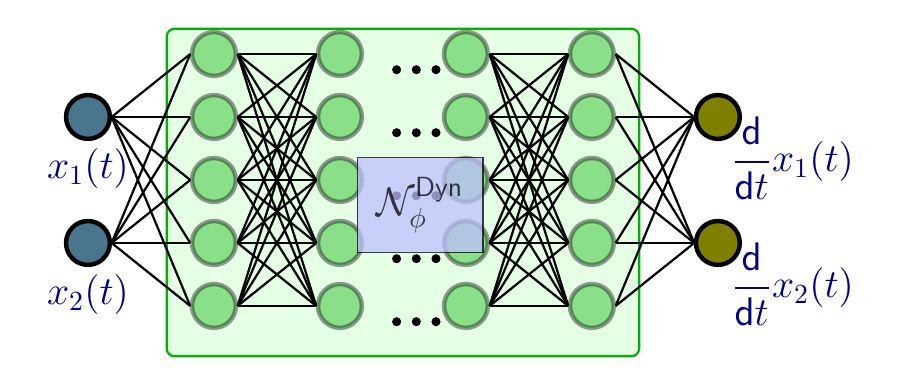
\begin{tikzpicture}[cir/.style={circle,draw=#1,minimum size=0.5},y=1cm,font=\sffamily, inner sep=7,transform shape,scale=1.0]
				\begin{scope}[rotate=0, scale = 0.8]
				\draw[draw=\fillcolorgreen, thick, rounded corners=.1cm, fill = green!10!white ] (-0.75,-4.8) rectangle ++(7.5,5.2);
				%%
				\node[cir=black,fill=cyan!50!black, draw = \boundarycolor,ultra thick] (I1) at (-2,-1) {};
				\node[cir=black,fill=cyan!50!black, draw = \boundarycolor,ultra thick] (I2) at (-2,-3) {};
				%						\node[cir=black,fill=red!50!black,draw = \boundarycolor,ultra thick] (I2) at (-2,-3) {};
				%%
				\node[cir=black,fill=\fillcolorgreen,draw = \boundarycolor,ultra thick, opacity=0.4] (a1) at (0,0) {};
				\node[cir=black,fill=\fillcolorgreen,opacity=0.4, draw = \boundarycolor,ultra thick] (a2) at (0,-1) {};
				\node[cir=black,fill=\fillcolorgreen,opacity=0.4,draw = \boundarycolor,ultra thick] (a3) at (0,-2) {};
				\node[cir=black,fill=\fillcolorgreen,opacity=0.4,draw = \boundarycolor,ultra thick] (a4) at (0,-3) {};
				\node[cir=black,fill=\fillcolorgreen,opacity=0.4,draw = \boundarycolor,ultra thick] (a5) at (0,-4) {};
				%%
				\node[cir=cyan!50!black,fill=\fillcolorgreen,opacity=0.4,draw = \boundarycolor,ultra thick] (b1) at (2,0) {};
				\node[cir=cyan!50!black,fill=\fillcolorgreen,opacity=0.4,draw = \boundarycolor,ultra thick] (b2) at (2,-1) {};
				\node[cir=cyan!50!black,fill=\fillcolorgreen,opacity=0.4,draw = \boundarycolor,ultra thick] (b3) at (2,-2) {};
				\node[cir=cyan!50!black,fill=\fillcolorgreen,opacity=0.4,draw = \boundarycolor,ultra thick] (b4) at (2,-3) {};
				\node[cir=cyan!50!black,fill=\fillcolorgreen,opacity=0.4,draw = \boundarycolor,ultra thick] (b5) at (2,-4) {};
				%%
				\node[cir=cyan!50!black,fill=\fillcolorgreen,opacity=0.4,draw = \boundarycolor,ultra thick] (c1) at (4,0) {};
				\node[cir=cyan!50!black,fill=\fillcolorgreen,opacity=0.4,draw = \boundarycolor,ultra thick] (c2) at (4,-1) {};
				\node[cir=cyan!50!black,fill=\fillcolorgreen,opacity=0.4,draw = \boundarycolor,ultra thick] (c3) at (4,-2) {};
				\node[cir=cyan!50!black,fill=\fillcolorgreen,opacity=0.4,draw = \boundarycolor,ultra thick] (c4) at (4,-3) {};
				\node[cir=cyan!50!black,fill=\fillcolorgreen,opacity=0.4,draw = \boundarycolor,ultra thick] (c5) at (4,-4) {};
				%%
				\node[cir=cyan!50!black,fill=\fillcolorgreen,opacity=0.4,draw = \boundarycolor,ultra thick] (d1) at (6,0) {};
				\node[cir=\boundarycolor,fill=\fillcolorgreen,opacity=0.4,draw = \boundarycolor,ultra thick] (d2) at (6,-1) {};
				\node[cir=\boundarycolor,fill=\fillcolorgreen,opacity=0.4,draw = \boundarycolor,ultra thick] (d3) at (6,-2) {};
				\node[cir=\boundarycolor,fill=\fillcolorgreen,opacity=0.4,draw = \boundarycolor,ultra thick] (d4) at (6,-3) {};
				\node[cir=\boundarycolor,fill=\fillcolorgreen,opacity=0.4,draw = \boundarycolor,ultra thick] (d5) at (6,-4) {};
				%%
				\node[cir=black,fill=green!50!red, draw = \boundarycolor,ultra thick] (O2) at (8,-3) {};
				\node[cir=black,fill=green!50!red, draw = \boundarycolor,ultra thick] (O1) at (8,-1) {};
				
				
				\foreach \i/\j in {a/b,c/d} {
					\foreach \cnto in {1,2,3,4,5} {
						\foreach \cntt in {1,2,3,4,5} {
							\draw[thick] (\i\cnto.east)--(\j\cntt.west);
						}
					}
				}
				
				\foreach \i/\j in {I/a} {
					\foreach \cnto in {1,2} {
						\foreach \cntt in {1,2,3,4,5} {
							\draw[thick] (\i\cnto.east)--(\j\cntt.west);
						}
					}
				}
				
				\foreach \i/\j in {d/O} {
					\foreach \cnto in {1,2,3,4,5} {
						\foreach \cntt in {1,2} {
							\draw[thick] (\i\cnto.east)--(\j\cntt.west);
						}
					}
				}
				
				\draw[decorate sep={1mm}{2.5mm},fill] (2.9,-0.25) -- (3.8,-0.25);
				\draw[decorate sep={1mm}{2.5mm},fill] (2.9,-1.25) -- (3.8,-1.25);
				\draw[decorate sep={1mm}{2.5mm},fill] (2.9,-2.25) -- (3.8,-2.25);
				\draw[decorate sep={1mm}{2.5mm},fill] (2.9,-3.25) -- (3.8,-3.25);
				\draw[decorate sep={1mm}{2.5mm},fill] (2.9,-4.25) -- (3.8,-4.25);		
				\end{scope}
				
				\draw (I1) node[blue!50!\boundarycolor,below=0.15cm] { \Large $x_1(t)$};
				\draw (I2) node[blue!50!\boundarycolor,below=0.15cm] { \Large $x_2(t)$};
				%					\draw (I2) node[blue!50!\boundarycolor,below=0.15cm] { \Large $\mathbf x$};
				\draw (O1) node[blue!50!\boundarycolor,below right=-0.25cm and -0.4cm] {\hspace{0.2cm} \Large $\dfrac{\d }{\d t} x_1(t)$};
				\draw (O2) node[blue!50!\boundarycolor,below right=-0.25cm and -0.4cm] {\hspace{0.2cm} \Large $\dfrac{\d }{\d t} x_2(t)$};
				
				\node (n1) [fill=blue!25,draw=black, below right = -0.5cm and 0cm of b3, opacity=0.75] {\Large $\mathcal{N}_\phi^{\textsf{Dyn}}$};     
				
				\end{tikzpicture}
				%%%%%%%%%%%%%%%%%%%%%%%%%%%%%%%%%%%%%%%%%%
			\end{tabular}
		};
		%%%%%%%%%%%%
		% RK part
%		\node[ fill = white,draw = green!50!black,  below right = 0cm and 8.5cm of implicit_respresentation.north, text = black, thick,rounded corners = 0.5ex, rotate = 0] (RKsteps) {
%			\begin{tabular}{c}
%				{\color{red!30!black} \huge Intergral constraint} \\[5pt]
%				%		\includegraphics[trim = 0cm 1.0cm 0cm 0.25cm, clip, scale = 0.4, angle = 0]{RK4_Steps.pdf}
%				$\mathbf x(t_j) \approx \mathbf x(t_i) + \int_{t_i}^{t_j}\mathbf g(\mathbf x(\tau))d\tau $
%				\vspace{-0.75cm}
%			\end{tabular}
%		};
		
		\node[ fill = none,draw = green!50!black,below left = 5.cm and -1.5cm  of implicit_respresentation.east, thick,rounded corners = 0.5ex, minimum width = .5cm, minimum height = .5cm] (loss) {\Large 
			\begin{tabular}{l}
				{\color{red!50!black} \huge Objective (loss) function :=} \\
				~~$\lambda_{\textsf{MSE}}\underbrace{\left\|\mathbf y_{\textsf{data}}(t) -  \mathcal{N}_\phi^{\textsf{Dyn}}(t) \mathbf x(t ) \right\|}_{\text{Implicit loss}}$ \\  ~~ + $\lambda_{\textsf{Integral}} \underbrace{\left\|\mathbf x(t_{j}) - \mathbf x(t_{i}) - \int_{t_i}^{t_j}\mathcal{N}_\phi^{\textsf{Dyn}}\left(\mathbf x (\tau)\right) d\tau\right\|}_{\text{prediction mismatch loss}}  $ \\ 
				~~ + $\lambda_{\textsf{Grad}}\underbrace{\left\|\dfrac{\d }{\d t} \mathbf x - \mathcal{N}_{\phi}^{\mathsf{Dyn}} (\mathbf x)  \right\|}_{\text{Gradient loss}}$,~~where $ \mathcal{N}_\phi^{\textsf{Dyn}}(t) =\mathbf x(t )$
			\end{tabular}
		};
		
				\node[ fill = white,draw = green!50!black, above  left =1cm and 8cm of loss.south, text = black, thick,rounded corners = 0.5ex] (denoised) {
			\begin{tabular}[t]{l}
				{\color{red!30!black} \huge Denoised data and learned neural dynamics ~~~~~~~~} \\[5pt]
				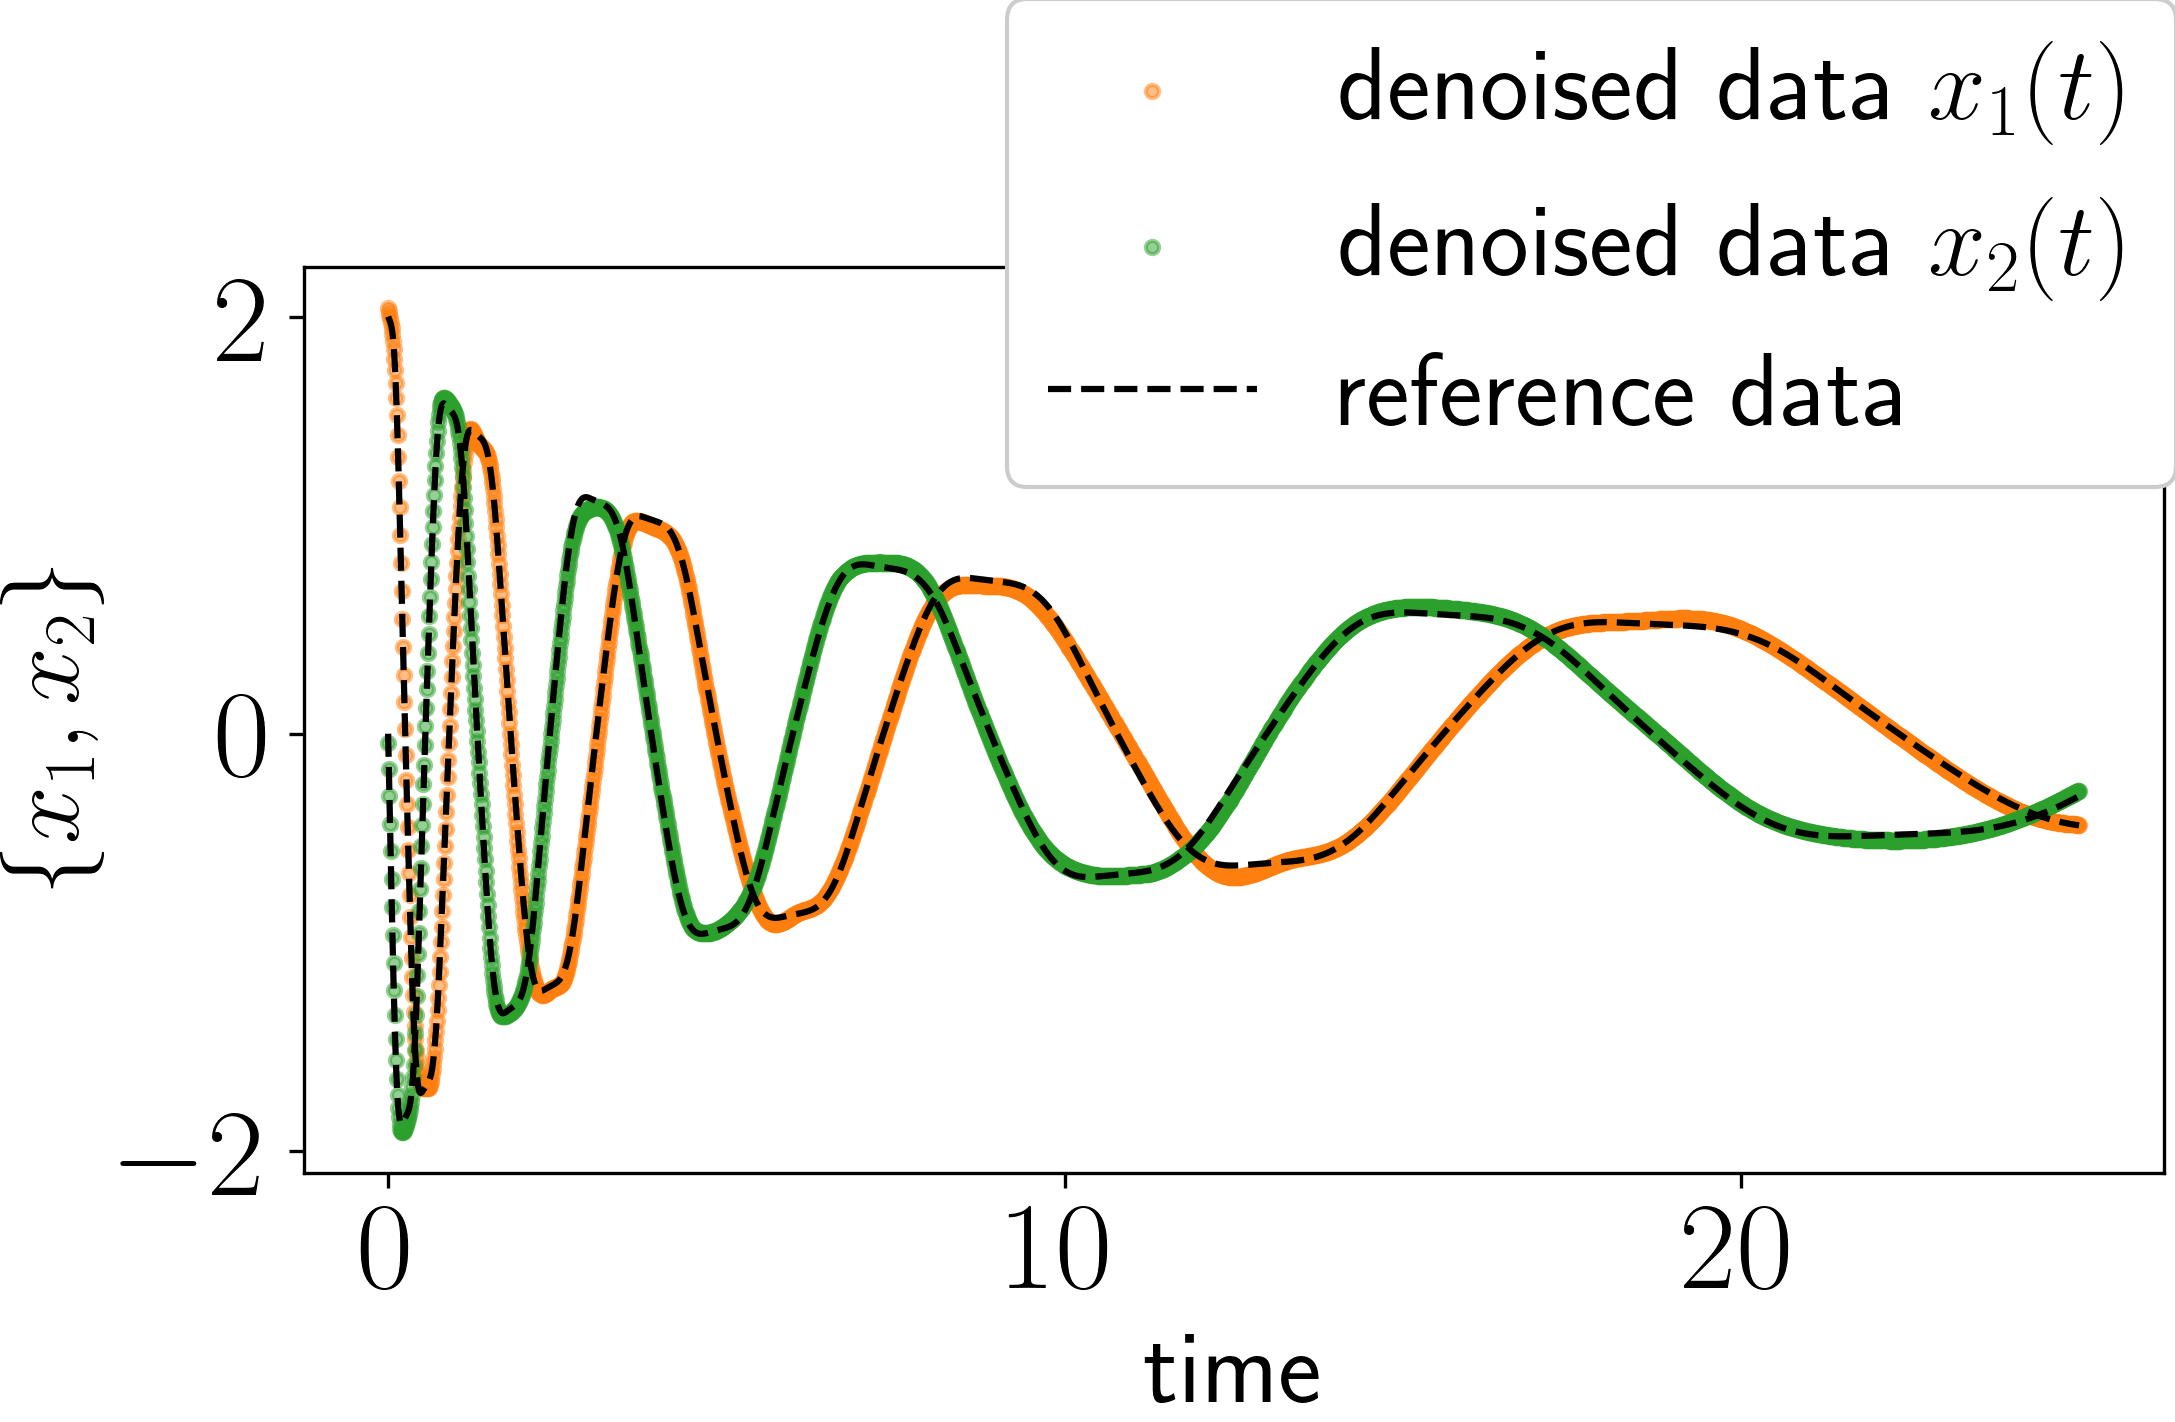
\includegraphics[trim = 0cm 0cm 0cm 0cm, clip, width = 8cm]{./main_diag2.pdf}
			\end{tabular}
		};
		
		\node[ fill = none,draw = none,below right = -3.2cm and 0.0cm  of burger, thick,rounded corners = 0.5ex, minimum width = .5cm, minimum height = .5cm] (arrow1) {
			\tikzfancyarrow[1.3cm]{{\Large ~~Data~~~}}
		};
	
		\node[ fill = none,draw = none, below right = 1.5cm and 0.7cm  of denoised.north, thick,rounded corners = 0.5ex, minimum width = 2cm, minimum height = .5cm] (arrow1) {\LARGE 
			\begin{tabular}{l}
				$	\mathbf x(t)  = \mathcal{N}_{\theta}^{\textsf{Imp}}(t)$,\\[2pt]
				and \\[2pt]
				$	\dfrac{\text{\sffamily{d}}}{\text{\sffamily{d}} t} {\mathbf x}(t)  \approx \mathcal{N}_{\phi}^{\textsf{Dyn}}(x(t))$
			\end{tabular}
		};
				\node[ fill = none,draw = none, above left =  -3.5cm and 2.75cm  of loss, thick,rounded corners = 0.5ex, minimum width = .5cm, minimum height = .5cm, rotate=-180] (arrow2) {
			\tikzfancyarrow[1.3cm]{{\rotatebox{180}{\Large Denoised}}}
		};
	\node[ fill = green!10!white,draw = green!50!black, above right =  3.0cm and 0.25cm  of burger.west, thick,rounded corners = 0.5ex, minimum width = .5cm, minimum height = .5cm] (a) {\Large a};
		\node[ fill = green!10!white,draw = green!50!black, above right =  3.0cm and 0.25cm  of implicit_respresentation.west, thick,rounded corners = 0.5ex, minimum width = .5cm, minimum height = .5cm] (b) {\Large b};
		%
%		\node[ fill = green!10!white,draw = green!50!black, above right =  7.5cm and 0.25cm  of RKsteps.south, thick,rounded corners = 0.5ex, minimum width = .5cm, minimum height = .5cm] (c) {\Large c};
		%
		\node[ fill = green!10!white,draw = green!50!black, above right =  2.25cm and 10.25cm  of loss.west, thick,rounded corners = 0.5ex, minimum width = .5cm, minimum height = .5cm] (c) {\Large c};
		\node[ fill = green!10!white,draw = green!50!black, above right =  2.75cm and 13.25cm  of denoised.west, thick,rounded corners = 0.5ex, minimum width = .5cm, minimum height = .5cm] (d) {\Large d};
	\end{tikzpicture}
\end{document}
